% !TeX Program=XeLaTeX
% !TeX root = surprises.tex

\chapter{מחוגה מתמוטטת}\label{c.collapse}

%%%%%%%%%%%%%%%%%%%%%%%%%%%%%%%%%%%%%%%%%%%%%%%%%%%%%%%%%%%%%%%

\vspace*{-2ex}

מחוגה מודרנית היא 
\textbf{מחוגה קבועה}:
ניתן לקבע את המרחק בין שתי הזרועות וכך להעתיק קטע קו או מעגל ממקום למקום (איור%
~\ref{fig.fixed-compass}).
אוקלידס השתמש במחוגה 
\textbf{מתמוטטת}
\L{(collapsing)}
שבה לא ניתן לשמור מרחק קבוע (איור%
~\ref{fig.collapsing-compass}),
שכן זרועותיה מתקפלות כאשר מרימים אותן מהנייר. לעיתים קרובות משתמשים מורים במחוגה מתמוטטת, המורכבת מטוש המחובר לחוט, כדי לבנות מעגל על הלוח. אי אפשר לשמור על מרחק קבוע כאשר מרחיקים את המחוגה מהלוח.

\begin{figure}[tb]
\begin{center}
\begin{subfigure}{.4\textwidth}
\centering
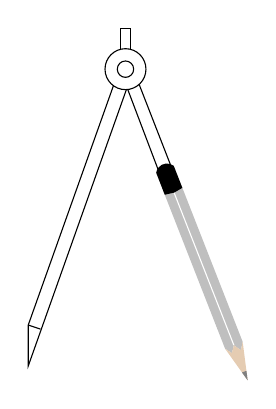
\begin{tikzpicture}
\begin{scope}[rotate=0,transform shape,scale=2.6]
\draw (2.95,3.7) rectangle (3,3.95);
\draw (2.92,3.68) -- (2.5,2.5) -- (2.5,2.3) -- (2.99,3.68);
\draw (3.5,2.5) -- (3.43,2.48) -- (2.975,3.68);
\draw (3.04,3.68) -- (3.5,2.5);
\draw (2.5,2.5) -- (2.56,2.48);
\draw[fill=white] (2.975,3.75) circle (0.1cm);
\draw (2.975,3.75) circle (0.04cm);
\end{scope}
\begin{scope}[xshift=9cm,yshift=6.2cm,rotate=21.4,scale=.6]          
\fill[gray!50] (0,4) -- (0.4,4) -- (0.4,0) --
               (0.3,-0.15) -- (0.2,0) -- (0.1,-0.14) --
               (0,0) -- cycle;
\draw[color=white] (0.2,4) -- (0.2,0);
\fill[black] (0,3.5) -- (0.2,3.47) -- (0.4,3.5) --
             (0.4,4) arc(30:150:0.23cm);
\fill[brown!40] (0,0) -- (0.2,-0.8)
    node[coordinate,pos=0.75](a){} -- 
    (0.4,0)node[coordinate,pos=0.25](b){} -- 
    (0.3,-0.15) -- (0.2,0) -- (0.1,-0.14) -- cycle;
\fill[gray] (a) -- (0.2,-0.8) -- (b) -- cycle;
\end{scope}
\end{tikzpicture}
\selectlanguage{hebrew}
\caption{מחוגה קבועה. לזרוע אחת סיכה שניתן להניח במרכז המעגל. עיפרון  המחובר לזרוע  השנייה משמש לשרטוט המעגל. הזרועות מחוברות בציר קשיח כך שהמרחק בין הזרועות (רדיוס המעגל) נשמר גם כאשר מרימים את המחוגה מהנייר.}
\label{fig.fixed-compass}
\end{subfigure}
\hspace{3em}
\begin{subfigure}[b]{.4\textwidth}
\centering
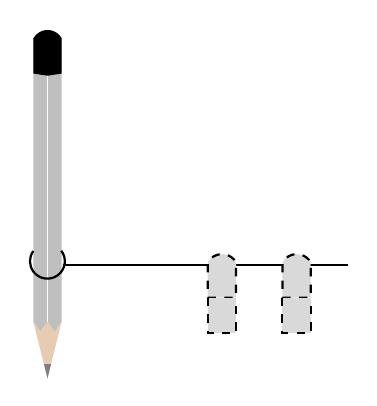
\begin{tikzpicture}[rotate=0,scale=.9]          
\fill[gray!50] (0,4) -- (0.4,4) -- (0.4,0) --
               (0.3,-0.15) -- (0.2,0) -- (0.1,-0.14) --
               (0,0) -- cycle;
\draw[color=white] (0.2,4) -- (0.2,0);
\fill[black] (0,3.5) -- (0.2,3.47) -- (0.4,3.5) --
             (0.4,4) arc(30:150:0.23cm);
\fill[brown!40] (0,0) -- (0.2,-0.8)
    node[coordinate,pos=0.75](a){} -- 
    (0.4,0) node[coordinate,pos=0.25](b){} -- 
    (0.3,-0.15) -- (0.2,0) -- (0.1,-0.14) -- cycle;
\fill[gray] (a) -- (0.2,-0.8) -- (b) -- cycle;

\draw[thick] (0.395,1) arc (37:-216:7pt);
\coordinate (knot) at (0.44,.8);
\draw[thick] (knot) -- +(4,0);
\fill (knot) circle (.7pt);

\begin{scope}[xshift=100pt,yshift=-90pt]
\draw[dashed,thick,fill=white!70!gray] (0,3.5) -- (0.4,3.5) -- 
      (0.4,4) arc(30:150:0.23cm) -- cycle;
\draw[dashed,thick,fill=white!70!gray] (0,3.5) -- ++(0,-.5) -- ++(.4,0) -- ++(0,.5);
\end{scope}

\begin{scope}[xshift=70pt,yshift=-90pt]
\draw[dashed,thick,fill=white!70!gray] (0,3.5) -- (0.4,3.5) -- 
      (0.4,4) arc(30:150:0.23cm) -- cycle;
\draw[dashed,thick,fill=white!70!gray] (0,3.5) -- ++(0,-.5) -- ++(.4,0) -- ++(0,.5);
\end{scope}
\end{tikzpicture}
\selectlanguage{hebrew}
\caption{%
מחוגה מתמוטטת. המשתמש מצמיד חוט למרכז המעגל. לקצה השני של החוט מחובר עיפרון המשמש לשרטוט המעגל. כאשר מרימים את המחוגה מהנייר, האצבעות (מקווקוות) עלולות להחליק בקלות למקום אחר.%
}\label{fig.collapsing-compass}
\end{subfigure}
\end{center}
\end{figure}

הפרק נפתח בדיון על הרלוונטיות של למידת בניות בסרגל ובמחוגה (סעיף%
~\ref{s.relevance}).
סעיף%
~\ref{s.collapse} 
משווה את שני סוגי המחוגה בבנייה הפשוטה ביותר: אנך אמצעי. סעיף%
~\ref{s.collapse-copy}
מביא את השיטה של אוקלידס להעתקת קטע קו באמצעות מחוגה מתמוטטת. שיטה זו מוכיחה שניתן לבצע באמצעות מחוגה מתמוטטת כל בנייה הניתנת לביצוע באמצעות מחוגה קבועה. סעיף%
~\ref{s.collapse-copy-incorrect} 
מציג הוכחה של משפט זה שנראית נכונה, אבל היא אינה נכונה עבור כל תצורה של קווים ונקודות. כדי להדגיש שאין לסמוך על שרטוט, סעיף%
~\ref{s.collapse-isoceles}
מביא את ה"הוכחה לכאורה" המפורסמת שכל משולש הוא שווה-שוקיים. ההוכחה נראית נכונה אבל היא שגויה כי היא מתבססת על שרטוט לא נכון.

%%%%%%%%%%%%%%%%%%%%%%%%%%%%%%%%%%%%%%%%%%%%%%%%%%%%%%%%%%%%%%%

\section{בנייה בסרגל ובמחוגה}\label{s.relevance}

עד לאחרונה בנייה בסרגל ובמחוגה הייתה מושג בסיסי שנלמד בגאומטרייה אוקלידית, אולם חשיבותה פחתה בסילבוסים מודרניים. מובן שלנושא אין כמעט חשיבות מעשית. כפי שאנו מראים בסעיפים%
~\ref{s.neusis}, \ref{s.neusis-doubling}, \ref{s.q}, \ref{s.square-quad},
היוונים ידעו לבנות בניות שאינן אפשריות בסרגל ובמחוגה, באמצעות כלים שהם רק מעט מתקדמים יותר. היום מסוגלים המחשבים לבצע בניות בדיוק רב ככל שנרצה באמצעות חישובים נומריים.

למרות זאת, אני מאמין שיש יתרונות ללימוד בניות בסרגל ובמחוגה:
\begin{itemize}
\item
מעניין יותר ומאתגר יותר ללמוד גאומטרייה דרך בניות לעומת קריאה של משפטים ושל הוכחות.
\item
התקדמויות מכריעות במתמטיקה הושגו במסגרת ניסיונות למצוא בניות. פרק%
~\ref{c.heptadecagon}
מביא בנייה של גאוס 
שהיוותה נקודת מוצא לאלגברה מודרנית, במיוחד התיאוריה שפותחה על ידי אוורסט גלואה 
\L{(\'{E}variste Galois)}.
\item
העובדה שיש בניות שאינן אפשריות קשה לעיכול ולכן מאוד מעניינת.
\item
מעציב שאנשים רבים מבזבזים שנים מחייהם בניסיון לבצע בניות שאינן אפשריות. חשוב שתלמידים יכירו שהמאמצים הללו חסרי תוחלת.
\end{itemize}


%%%%%%%%%%%%%%%%%%%%%%%%%%%%%%%%%%%%%%%%%%%%%%%%%%%%%%%%%%%%%%%

\section{מחוגה קבועה ומחוגה מתמוטטת}\label{s.collapse}

בספרי לימוד גאומטרייה ניתן למצוא בנייה של אנך אמצעי לקטע קו על ידי בניית שני מעגלים שמרכזם על הקו, ובלבד שהרדיוס גדול ממחצית המרחק בין המרכזים 
(איור%
~\ref{f.collapse-perp-bisector-fixed}).
בנייה זו אפשרית רק בעזרת מחוגה קבועה, כי לאחר בניית המעגל שמרכזו 
$A$,
המרחק בין זרועות המחוגה חייב להישאר ללא שינוי כדי לבנות את המעגל שמרכזו 
$B$.

איור%
~\ref{f.collapse-perp-bisector-collapse}
מראה בנייה של אנך אמצעי הפועלת גם עם מחוגה קבועה וגם עם מחוגה מתמוטטת. נבנה שני מעגלים: אחד שמרכזו 
$A$
עם רדיוס
$\overline{AB}$
ואחד שמרכזו B עם רדיוס
$\overline{BA}$.
הבנייה אפשרית עם מחוגה מתמוטטת כי (ברור)
$\overline{AB}=\overline{BA}$,
ולכן המחוגה לא חייבת "לזכור" את האורך של
$\overline{AB}$
כדי לבנות מעגל שמרכזו 
$B$
עם רדיוס זהה.

הוכחת הנכונות של הבנייה באיור%
~\ref{f.collapse-perp-bisector-fixed}
אינה פשוטה כלל, כי חייבים להשתמש במושגים יחסית מתקדמים כגון משולשים חופפים. אבל הוכחת הנכונות של הבנייה באיור%
~\ref{f.collapse-perp-bisector-collapse}
פשוטה ומבוססת על העובדה ש-%
$\triangle ABC$
הוא משולש שווה-צלעות. טענה זו היא המשפט הראשון בספר של אוקלידס. 
$\overline{AC}=\overline{AB}$
כי הם רדיוסים של אותו מעגל, וכן
$\overline{BC}=\overline{BA}$.
מכאן:
$\overline{AC} = \overline{AB} = \overline{BA} = \overline{BC}$.

איור%
~\ref{f.collapse-equilateral-fixed}
מראה שעבור הבנייה במחוגה קבועה, המשולש יהיה שווה-שוקיים אך לא בהכרח שווה-צלעות 
(איור~
\ref{f.collapse-equilateral-collapse}).

%%%%%%%%%%%%%%%%%%%%%%%%%%%%%%%%%%%%%%%%%%%%%%%%%%%%%%%%%%%%%%%


\section{העתקת קטע קו לפי אוקלידס}\label{s.collapse-copy}

המשפט השני בספרו של אוקלידס מתאר איך להעתיק קטע קו נתון
$\overline{AB}$
לקטע באותו אורך שאחת מנקודות הקצה שלו היא נקודה נתונה
$C$.
מכאן שמחוגה קבועה אינה מוסיפה יכולות ואפשר להסתפק במחוגה מתמוטטת, אבל הבניות יהיו מסובכות יותר.

\begin{theorem}
נתון קטע
$\overline{AB}$
ונקודה
$C$,
ניתן לבנות במחוגה מתמוטטת קטע 
$\overline{CC'}$
שאחת מנקודות הקצה שלו היא
$C$
ואורכו
$\overline{AB}=\overline{CC'}$ 
(איור~
\ref{f.collapse-copying-1}).
\end{theorem}

\begin{figure}[t]
\begin{center}
\begin{subfigure}{.4\textwidth}
\centering
\begin{tikzpicture}[scale=0.5]
\coordinate (A) at (0,0);
\coordinate (B) at (4,0);
\vertex{A};
\vertex{B};
\draw (A) node[below left] {$A$} -- (B) node[below right] {$B$};
\draw[name path=larc] (A) ++(-60:3cm) arc (-60:60:3cm);
\draw[name path=rarc] (B) ++(-120:3cm) arc (-120:-240:3cm);
\path [name intersections={of=larc and rarc,by={b,t}}];
\node[above right,xshift=-2pt,yshift=5pt] at (t) {$C$};
\node[below left,xshift=2pt,yshift=-5pt] at (b) {$D$};
\draw ($ (b) ! 1.2 ! (t)$) -- ($ (t) ! 1.2 ! (b)$);
\end{tikzpicture}
\selectlanguage{hebrew}
\caption{בניית אנך אמצעי בעזרת מחוגה קבועה}\label{f.collapse-perp-bisector-fixed}
\end{subfigure}
\hfill
\begin{subfigure}{.4\textwidth}
\centering
\begin{tikzpicture}[scale=0.5]
\coordinate (A) at (0,0);
\coordinate (B) at (4,0);
\vertex{A};
\vertex{B};
\draw (A) node[below left] {$A$} -- (B) node[below right] {$B$};
\draw[name path=larc] (A) ++(-80:4cm) arc (-80:80:4cm);
\draw[name path=rarc] (B) ++(-100:4cm) arc (-100:-260:4cm);
\path [name intersections={of=larc and rarc,by={b,t}}];
\node[above right,xshift=-2pt,yshift=3pt] at (t) {$C$};
\node[below left,xshift=2pt,yshift=-3pt] at (b) {$D$};
\draw ($ (b) ! 1.2 ! (t)$) -- ($ (t) ! 1.2 ! (b)$);
\end{tikzpicture}
\selectlanguage{hebrew}
\caption{בניית אנך אמצעי בעזרת מחוגה מתמוטטת}\label{f.collapse-perp-bisector-collapse}
\end{subfigure}
\end{center}
\end{figure}


\begin{figure}[b]
\begin{center}
\begin{subfigure}{.4\textwidth}
\centering
\begin{tikzpicture}[scale=0.5]
\coordinate (A) at (0,0);
\coordinate (B) at (4,0);
\vertex{A};
\vertex{B};
\draw (A) node[below left] {$A$} -- (B) node[below right] {$B$};
\draw[name path=larc] (A) ++(-60:3cm) arc (-60:60:3cm);
\draw[name path=rarc] (B) ++(-120:3cm) arc (-120:-240:3cm);
\path [name intersections={of=larc and rarc,by={b,t}}];
\vertex{t};
\vertex{b};
\node[above right,xshift=-2pt,yshift=5pt] at (t) {$C$};
\node[below left,xshift=2pt,yshift=-5pt] at (b) {$D$};
\draw (A) -- (t);
\draw (B) -- (t);
\end{tikzpicture}
\selectlanguage{hebrew}
\caption{בניית משולש שווה-שוקיים בעזרת מחוגה קבועה}\label{f.collapse-equilateral-fixed}
\end{subfigure}
\hspace{3em}
\begin{subfigure}{.4\textwidth}
\centering
\begin{tikzpicture}[scale=0.5]
\coordinate (A) at (0,0);
\coordinate (B) at (4,0);
\draw (A) node[below left] {$A$} -- (B) node[below right] {$B$};
\vertex{A};
\vertex{B};
\draw[name path=larc] (A) ++(-80:4cm) arc (-80:80:4cm);
\draw[name path=rarc] (B) ++(-100:4cm) arc (-100:-260:4cm);
\path [name intersections={of=larc and rarc,by={b,t}}];
\vertex{t};
\vertex{b};
\node[above right,xshift=-2pt,yshift=3pt] at (t) {$C$};
\node[below left,xshift=2pt,yshift=-3pt] at (b) {$D$};
\draw (A) -- (t);
\draw (B) -- (t);
\end{tikzpicture}
\selectlanguage{hebrew}
\caption{בניית משולש שווה-צלעות בעזרת מחוגה קבועה או מחוגה מתמוטטת}\label{f.collapse-equilateral-collapse}
\end{subfigure}
\end{center}
\end{figure}

\begin{figure}[t]
\begin{center}
\begin{subfigure}{.4\textwidth}
\centering
\begin{tikzpicture}[scale=0.5]
\coordinate (C) at (0,0);
\coordinate (A) at (3,0);
\draw (A) node[below,xshift=-2pt,yshift=-2pt] {$A$} -- +(40:4) coordinate (B) node[right] {$B$};
\vertex{A};
\vertex{B};
\vertex{C};
\node[below,xshift=2pt,yshift=-2pt] at (C) {$C$};
\draw[thick,dashed] (C) -- +(160:4) coordinate (D) node[below] {$C'$};
\vertex{D};
\end{tikzpicture}
\selectlanguage{hebrew}
\caption{העתקת קטע קו $\overline{AB}$}\label{f.collapse-copying-1}
\end{subfigure}
\hspace{3ex}
\begin{subfigure}{.4\textwidth}
\centering
\begin{tikzpicture}[scale=0.5]
\coordinate (C) at (0,0);
\coordinate (A) at (3,0);
\draw (A) node[below,xshift=-2pt,yshift=-2pt] {$A$} -- +(40:4) coordinate (B) node[right] {$B$};
\vertex{B};
\node[below,xshift=2pt,yshift=-2pt] at (C) {$C$};
\draw (A) -- (C);
\path[name path=larc] (C) ++(-70:2.5cm) arc (-70:70:2.5cm);
\path[name path=rarc] (A) ++(-110:2.5cm) arc (-110:-250:2.5cm);
\path [name intersections={of=larc and rarc,by={d,D}}];
\node[above] at (D) {$D$};
\draw (A) -- (D);
\draw (C) -- (D);
\end{tikzpicture}
\selectlanguage{hebrew}
\caption{העתקת קטע קו בעזרת מחוגה מתמוטטת}\label{f.collapse-copying-2}
\end{subfigure}
\end{center}
\end{figure}

\begin{proof}
נבנה קטע 
$\overline{AC}$
ומשולש שווה-צלעות 
$\triangle ACD$
שבסיסו
$\overline{AC}$
(איור~
\ref{f.collapse-copying-2}).
לפי המשפט הראשון של אוקלידס הבנייה אפשרית באמצעות מחוגה מתמוטטת. נבנה קרן שהיא המשך הקטע מ-%
$D$
לכיוון 
$A$,
ונבנה קרן שהיא המשך הקטע מ-
$D$
לכיוון
$C$
(איור~
\ref{f.collapse-copying-3}).

נבנה מעגל שמרכזו 
$A$
עם רדיוס
$\overline{AB}$,
ונסמן ב-%
$E$
את נקודת החיתוך של המעגל עם הקרן שממשיכה את
$\overline{DA}$
(איור~
\ref{f.collapse-copying-4}).
נבנה מעגל שמרכזו 
$D$
עם רדיוס 
$\overline{DE}$,
ונסמן ב-%
$F$
את נקודת החיתוך של המעגל עם הקרן שממשיכה את
$\overline{DC}$
(איור%
~\ref{f.collapse-copying-5}).

\begin{figure}[b]
\begin{center}
\begin{subfigure}{.4\textwidth}
\centering
\begin{tikzpicture}[scale=0.6]
\coordinate (C) at (0,0);
\coordinate (A) at (2.5,0);
\coordinate (B) at (5.5,2);
\draw (A) node[below,xshift=-2pt,yshift=-2pt] {$A$} -- (B) node[right] {$B$};
%\fill (A) circle[radius=3pt];
%\fill (B) circle[radius=3pt];
\node[below,xshift=2pt,yshift=-2pt] at (C) {$C$};
\draw (A) -- (C);
\path[name path=larc] (C) ++(-70:2.5cm) arc (-70:70:2.5cm);
\path[name path=rarc] (A) ++(-110:2.5cm) arc (-110:-250:2.5cm);
\path [name intersections={of=larc and rarc,by={d,D}}];
\node[above] at (D) {$D$};
\draw (A) -- (D);
\draw (C) -- (D);
\draw[name path=ray2] (D) -- ($ (D) ! 2.7 ! (C) $);
\draw[name path=ray1] (D) -- ($ (D) ! 2.7 ! (A) $);
\end{tikzpicture}
\selectlanguage{hebrew}
\caption{בניית קרניים מ-%
$D$}\label{f.collapse-copying-3}
\end{subfigure}
\hspace{3ex}
\begin{subfigure}{.4\textwidth}
\centering
\begin{tikzpicture}[scale=0.6]
\coordinate (C) at (0,0);
\coordinate (A) at (2.5,0);
\coordinate (B) at (5.5,2);
\draw (A) node[below,xshift=-2pt,yshift=-2pt] {$A$} -- (B) node[right] {$B$};
%\fill (A) circle[radius=3pt];
%\fill (B) circle[radius=3pt];
%\fill (C) node[below,xshift=2pt,yshift=-2pt] {$C$} circle[radius=3pt];
\node[below,xshift=2pt,yshift=-2pt] at (C) {$C$};
\draw (A) -- (C);
\path[name path=larc] (C) ++(-70:2.5cm) arc (-70:70:2.5cm);
\path[name path=rarc] (A) ++(-110:2.5cm) arc (-110:-250:2.5cm);
\path [name intersections={of=larc and rarc,by={d,D}}];
%\fill (D) node[above] {$D$} circle[radius=3pt];
\node[above] at (D) {$D$};
\draw (A) -- (D);
\draw (C) -- (D);
\draw[name path=ray2] (D) -- ($ (D) ! 2.7 ! (C) $);
\draw[name path=ray1] (D) -- ($ (D) ! 2.7 ! (A) $);
\node[draw,circle through=(B),name path=c1] at (A) {};
\path [name intersections={of=c1 and ray1,by={E,e}}];
%\fill (E) node[right,xshift=2pt,yshift=-2pt] {$E$} circle[radius=3pt];
\node[right,xshift=2pt,yshift=-2pt] at (E) {$E$};
\end{tikzpicture}
\selectlanguage{hebrew}
\caption{מעגל עם רדיוס 
$\overline{AB}$}\label{f.collapse-copying-4}
\end{subfigure}
\end{center}
\end{figure}

\begin{figure}[tb]
\begin{center}
\begin{tikzpicture}[scale=0.4]
\coordinate (C) at (0,0);
\coordinate (A) at (2.5,0);
\coordinate (B) at (5.5,2);
\draw (A) node[below,xshift=-2pt,yshift=-2pt] {$A$} -- (B) node[right] {$B$};
%\fill (A) circle[radius=3pt];
%\fill (B) circle[radius=3pt];
%\fill (C) node[below,xshift=2pt,yshift=-2pt] {$C$} circle[radius=3pt];
\node[below,xshift=2pt,yshift=-2pt] at (C) {$C$};
\draw (A) -- (C);
\path[name path=larc] (C) ++(-70:2.5cm) arc (-70:70:2.5cm);
\path[name path=rarc] (A) ++(-110:2.5cm) arc (-110:-250:2.5cm);
\path [name intersections={of=larc and rarc,by={d,D}}];
%\fill (D) node[above] {$D$} circle[radius=3pt];
\node[above] at (D) {$D$};
\draw (A) --  (D);
\draw (C) --  (D);
\draw[name path=ray2] (D) -- ($ (D) ! 3 ! (C) $);
\draw[name path=ray1] (D) -- ($ (D) ! 3 ! (A) $);
\node[draw,circle through=(B),name path=c1] at (A) {};
\path [name intersections={of=c1 and ray1,by={E,e}}];
%\fill (E) node[right,xshift=2pt,yshift=-2pt] {$E$} circle[radius=3pt];
\node[right,xshift=2pt,yshift=-2pt] at (E) {$E$};
\node[draw,circle through=(E),name path=c2] at (D) {};
\path [name intersections={of=c2 and ray2,by={F,f}}];
%\fill (F) node[left,xshift=-2pt,yshift=-2pt] {$F$} circle[radius=3pt];
\node[left,xshift=-2pt,yshift=-2pt] at (F) {$F$};
\path (A) -- node[right] {$a$} (E);
\path (C) -- node[left] {$a$} (F);
\end{tikzpicture}
\selectlanguage{hebrew}
\caption{בניית $\overline{CF}=\overline{AB}$}\label{f.collapse-copying-5}
\end{center}
\end{figure}

$\overline{DC}=\overline{DA}$
כי
$\triangle ACD$
שווה-צלעות.
$\overline{AE}=\overline{AB}$
כי שניהם רדיוסים של המעגל שמרכזו 
$A$,
וכן
$\overline{DF}=\overline{DE}$.
מכאן:
\[
\overline{CF} = \overline{DF} - \overline{DC} = \overline{DE} - \overline{DC} = \overline{DE} - \overline{DA} = \overline{AE} = \overline{AB}\,.
\].
\end{proof}

הדרישה על כיוון הקרנות חיונית. הוכחה זו נכונה לכל קטע קו
$\overline{AB}$
ולכל נקודה
$C$,
ללא תלות במיקום שלה יחסית ל-%
$\overline{AB}$.
בגלל דרישת הכיוון של הקרנות, ה"חרוט" הכלוא בין שתי הקרנות יחתוך את המעגלים גם אם
$\overline{AC}>\overline{AB}$
(איור%
~\ref{f.collapse-copying-6}).

\begin{figure}[tb]
\begin{center}
\begin{tikzpicture}[scale=0.3]
\clip (-12,-6) rectangle (11,10);
\coordinate (C) at (-4,0);
\coordinate (A) at (3,0);
\draw (A) node[below,xshift=-2pt,yshift=-2pt] {$A$} -- +(40:4) coordinate (B) node[right] {$B$};
\node[below,xshift=2pt,yshift=-2pt] at (C) {$C$};
\draw (A) -- (C);
\path[name path=larc] (C) ++(-70:7cm) arc (-70:70:7cm);
\path[name path=rarc] (A) ++(-110:7cm) arc (-110:-250:7cm);
\path [name intersections={of=larc and rarc,by={d,D}}];
\node[above] at (D) {$D$};
\draw (A) -- (D);
\draw (C) -- (D);
\draw[name path=ray2] (D) -- ($ (D) ! 2 ! (C) $);
\draw[name path=ray1] (D) -- ($ (D) ! 2 ! (A) $);
\node[draw,circle through=(B),name path=c1] at (A) {};
\path [name intersections={of=c1 and ray1,by={e,E}}];
\node[right,xshift=2pt,yshift=-2pt] at (E) {$E$};
\node[draw,circle through=(E),name path=c2] at (D) {};
\path [name intersections={of=c2 and ray2,by={F,f}}];
\node[left,xshift=-2pt,yshift=-2pt] at (F) {$F$};
\path (A) -- node[right] {$a$} (E);
\path (C) -- node[left] {$a$} (F);
\draw[white,fill=white] (-12,8) rectangle +(23,2);
\end{tikzpicture}
\end{center}
\selectlanguage{hebrew}
\caption{בנייה עבור $\overline{AC}>\overline{AB}$}\label{f.collapse-copying-6}
\end{figure}

%%%%%%%%%%%%%%%%%%%%%%%%%%%%%%%%%%%%%%%%%%%%%%%%%%%%%%%%%%%%%%%

\section{העתקה שגויה של קטע}\label{s.collapse-copy-incorrect}

\begin{proof}

נבנה שלושה מעגלים: מעגל שמרכזו
$A$
עם רדיוס
$\overline{AB}$,
מעגל שמרכזו
$A$
עם רדיוס
$\overline{AC}$
ומעגל שמרכזו
$C$
עם רדיוס
$\overline{AC}=\overline{CA}$.
נסמן את נקודות החיתוך של המעגלים בעלי הרדיוסים השווים 
ב-%
$E,F$.
נסמן ב-D את נקודת החיתוך של המעגל שמרכזו
$C$
עם המעגל ברדיוס AB שמרכזו 
$A$.

עבור
$\overline{AC}>\overline{AB}$,
הבנייה מוצגת באיור%
~\ref{f.collapse-incorrect-1}.
\begin{figure}[tb]
\begin{center}
\begin{tikzpicture}[scale=0.45]
\coordinate (C) at (-2,0);
\coordinate (A) at (2.5,0);
\coordinate (B) at (4.5,1.5);
\draw (A) node[below right] {$A$} -- (B) node[right] {$B$};
%\fill (A) circle[radius=3pt];
%\fill (B) circle[radius=3pt];
\fill (C) node[left,xshift=-2pt] {$C$} circle[radius=3pt];
\node[draw,circle through=(B),name path=c1] at (A) {};
\node[draw,circle through=(C),name path=c2] at (A) {};
\node[draw,circle through=(A),name path=c3] at (C) {};
\path [name intersections={of=c1 and c3,by={D,f}}];
\path [name intersections={of=c2 and c3,by={E,F}}];
%\fill (D) node[below right,xshift=4pt] {$D$} circle[radius=3pt];
%\fill (E) node[above,yshift=2pt] {$E$} circle[radius=3pt];
%\fill (F) node[below,yshift=-2pt] {$F$} circle[radius=3pt];
\node[below right,xshift=4pt] at (D) {$D$};
\node[above,yshift=2pt] at (E) {$E$};
\node[below,yshift=-2pt] at (F) {$F$};
\end{tikzpicture}
\selectlanguage{hebrew}
\end{center}
\caption{בנייה עבור העתקת קטע (1)}\label{f.collapse-incorrect-1}
\end{figure}

נבנה מעגל שמרכזו 
$E$
עם רדיוס 
$\overline{ED}$.
נסמן ב-%
$G$
את נקודת החיתוך של מעגל זה עם המעגל ברדיוס AC ששמרכזו
$A$.

יש שתי נקודות חיתוך, נבחר את הנקודה הקרובה יותר ל-%
$C$
(איור~%
\ref{f.collapse-incorrect-2}).

$\overline{CD}=\overline{CE}$
הם רדיוסים באותו מעגל, כך גם
$\overline{AE}=\overline{AG}$.
לפי הבנייה הרדיוסים 
$\overline{CE}$
ו-%
$\overline{AE}$
שווים. מכאן:
\[
\overline{CD} = \overline{CE} = \overline{AE} = \overline{AG}\,.
\]

\newpage

$\overline{EG} = \overline{ED}$
הם רדיוסים באותו מעגל, ולכן
$\triangle EAG\cong \triangle DCE$
לפי צלע,צלע,צלע ו-%
$\angle GEA = \angle DEC$.

מכיוון ש:
\[
\angle GEC = \angle GEA \!-\!\angle CEA = \angle DEC\!-\!\angle CEA = \angle DEA\,,
\]
$\triangle ADE\cong\triangle CGE$ 
לפי צלע, זווית, צלע.
$\overline{AB}=\overline{AD}$
הם רדיוסים במעגל שמרכזו
$A$,
ולכן
$\overline{GC}=\overline{AD}=\overline{AB}$.
\end{proof}

\begin{figure}[tb]
\begin{center}
\begin{tikzpicture}[scale=0.6]
\clip (-8,-1) rectangle (9,5);
\coordinate (C) at (-2,0);
\coordinate (A) at (2.5,0);
\coordinate (B) at (4.5,1.5);
\draw[thick] (A) node[below right] {$A$} -- (B) node[right] {$B$};
\vertex{A};
\vertex{C};
\node[below left] at (C) {$C$};
\node[draw,circle through=(B),name path=c1] at (A) {};
\node[draw,circle through=(C),name path=c2] at (A) {};
\node[draw,circle through=(A),name path=c3] at (C) {};
\path [name intersections={of=c1 and c3,by={D,f}}];
\path [name intersections={of=c2 and c3,by={E,F}}];
\node[draw,circle through=(D),name path=c4] at (E) {};
\path [name intersections={of=c2 and c4,by={g,G}}];
\node[left] at (G) {$G$};
\node[below right,yshift=2pt,xshift=2pt] at (D) {$D$};
\node[above] at (E) {$E$};
\vertex{E};
\vertex{F};
\draw (C) -- (G);
\draw (A) -- (G) -- (E) -- (C) -- (D);
\draw (A) -- (D) -- (E) -- cycle;
\end{tikzpicture}
\end{center}
\selectlanguage{hebrew}
\caption{בנייה עבור העתקת קטע (2)}\label{f.collapse-incorrect-2}
\end{figure}

הבנייה נכונה רק אם
$\overline{AC}>\overline{AB}$.
באיור%
~\ref{f.collapse-incorrect-4}
מתואר המקרה שבו
$\overline{AC}<\overline{A}B$
, ואפשר לראות ש-%
$\overline{AB}\neq\overline{GC}$.

\begin{figure}[tb]
\begin{center}
\begin{tikzpicture}[scale=0.6]
\coordinate (C) at (-1,0);
\coordinate (A) at (2,0);
\coordinate (B) at (6,1.5);
\draw[thick] (A) node[below right] {$A$} -- (B) node[right] {$B$};
\node[left,xshift=-2pt] at (C) {$C$};
\node[draw,circle through=(B),name path=c1] at (A) {};
\node[draw,circle through=(C),name path=c2] at (A) {};
\node[draw,circle through=(A),name path=c3] at (C) {};
\path [name intersections={of=c1 and c3,by={D,f}}];
\path [name intersections={of=c2 and c3,by={E,F}}];
\node[above left,xshift=4pt] at (D) {$D$};
\node[above,yshift=2pt] at (E) {$E$};
\node[below,yshift=-2pt] at (F) {$F$};
\vertex{A};
\vertex{C};
\node[draw,circle through=(D),name path=c4] at (E) {};
\path [name intersections={of=c2 and c4,by={g,G}}];
\node[right,xshift=2pt,yshift=2pt] at (G) {$G$};
\draw[thick] (G) -- (C);
\end{tikzpicture}
\selectlanguage{hebrew}
\caption{תרשים שעבורו ההוכחה לא עובדת}\label{f.collapse-incorrect-4}
\end{center}
\end{figure}

%%%%%%%%%%%%%%%%%%%%%%%%%%%%%%%%%%%%%%%%%%%%%%%%%%%%%%%%%%%%%%%

\section{אין לסמוך על תרשים}\label{s.collapse-isoceles}

\begin{theorem}
\textbf{(שגוי, כמובן)}
כל משולש הוא שווה-שוקיים.
\end{theorem}

\begin{figure}[tb]
\begin{center}
\begin{tikzpicture}[scale=1.2]
\coordinate (P) at (0,0);
\node[xshift=4mm,yshift=1mm] at (P) {$P$};
\coordinate [label=left:$B$] (B)  at (-2,-2);
\coordinate [label=right:$C$] (C)  at (4,-2);
\coordinate [label=above:$A$] (A)  at (-1,2);
\node[below,yshift=-12pt,xshift=2pt] at (A) {$\alpha$};
\node[below,yshift=-12pt,xshift=15pt] at (A) {$\alpha$};
\draw (A) -- (B);
\draw (A) -- (C);
\draw (B) -- (C);
\draw (A) -- (P);
\draw (B) -- (P);
\draw (C) -- (P);
\coordinate[label=left:$E$] (E) at ($ (A) ! .44 ! (B) $);
\draw[rotate=-100] (E) rectangle +(8pt,8pt);
\draw (P) -- (E);
\coordinate[label=right:$F$] (F) at ($ (A) ! .33 ! (C) $);
\draw[rotate=-132] (F) rectangle +(8pt,8pt);
\draw (P) -- (F);
\coordinate[label=below:$D$] (D) at ($ (B) ! .33 ! (C) $);
\draw (D) rectangle +(8pt,8pt);
\draw (P) -- (D);
\node[left] at ($ (A) ! .5 ! (E) $) {};
\node[left] at ($ (B) ! .5 ! (E) $) {};
\node[below] at ($ (B) ! .5 ! (D) $) {$a$};
\node[below] at ($ (C) ! .5 ! (D) $) {$a$};
\node[right,xshift=2pt] at ($ (A) ! .5 ! (F) $) {};
\node[right,xshift=2pt] at ($ (C) ! .5 ! (F) $) {};
%\fill (A) circle(1pt);
%\fill (B) circle(1pt);
%\fill (C) circle(1pt);
\fill (D) circle(1pt);
\fill (E) circle(1pt);
\fill (F) circle(1pt);
\fill (P) circle(1pt);
\end{tikzpicture}
\selectlanguage{hebrew}
\caption{הוכחה שגויה שכל משולש הוא שווה-שוקיים}\label{f.isoceles}
\end{center}
\end{figure}
\begin{proof}
נתון משולש שרירותי 
$\triangle ABC$.
תהי
$P$
נקודת החיתוך של חוצה הזווית 
$\angle BAC$
והאנך האמצעי של 
$\overline{BC}$.
נקודות החיתוך של הגבהים מ-%
$P$
לצלעות
$\overline{AB},\overline{AC}$
מסומנים ב-%
$E,F$
בהתאמה (איור
\ref{f.isoceles}).
$\triangle APE\cong \triangle APF$
כי הם משולשים ישרי-זווית שבהם זוויות שוות
$\alpha$
וצלע משותפת
$\overline{AP}$.
$\triangle DPB\cong \triangle DPC$
כי הם משולשים ישרי-זווית,
$\overline{PD}$
צלע משותפת ו-%
$\overline{BD}=\overline{DC}=a$.
$\triangle EPB\cong \triangle FPC$
כי הם משולשים ישרי-זווית,
$\overline{EP}=\overline{PF}$
לפי החפיפה הראשונה, ו-%
$\overline{PB}=\overline{PC}$
לפי החפיפה השנייה. מהשוויונות נקבל ש-%
$\triangle ABC$
שווה-שוקיים:
\[
\overline{AB}=\overline{AE}+\overline{EB}=\overline{AF}+\overline{FC}=\overline{AC}\,.
\]
\end{proof}

ה"לוגיקה" של ההוכחה נכונה, אך ההוכחה מבוססת על תרשים שאינו נכון, כי הנקודה
$P$
נמצאת מחוץ למשולש (איור%
~\ref{f.isoceles-wrong}).
\begin{figure}[tb]
\begin{center}
\begin{tikzpicture}[scale=.7]
\coordinate (B)  at (0,0);
\node[left] at (B) {$B$};
\coordinate (C)  at (7,0);
\node[right] at (C) {$C$};
\path[name path=pathb] (B) -- +(80:6.5);
\path[name path=pathc] (C) -- +(140:9.5);
\path [name intersections={of=pathb and pathc,by={A}}];
\node[above] at (A) {$A$};
%\fill (A) circle(1pt) node[above] {$A$};
%\fill (B) circle(1pt) node[left] {$B$};
%\fill (C) circle(1pt) node[right] {$C$};
\draw (A) -- (B) -- (C) -- cycle;
\draw[name path=angle] (A) -- +(-70:8.5);
\draw ($(B)!.5!(C)$) |- +(0,4);
\draw[name path=perp] ($(B)!.5!(C)$) |- +(0,-3);
\draw ($(B)!.5!(C)$) rectangle +(8pt,8pt);
\path [name intersections={of=angle and perp,by={P}}];
\fill (P) circle(2pt) node[right] {$P$};
\node[below,yshift=-12pt,xshift=2pt] at (A) {$\alpha$};
\node[below,yshift=-12pt,xshift=15pt] at (A) {$\alpha$};
\end{tikzpicture}
\selectlanguage{hebrew}
\caption{הסיבה לכך שהבנייה לא עובדת}\label{f.isoceles-wrong}
\end{center}
\end{figure}

\subsection*{מה ההפתעה?}

כתלמיד, הנחתי כמובן מאליו שלמחוגה יש ציר חיכוך השומר על המרחק בין החוד לעיפרון. הכאשר המורה השתשמשה במחוגה המורכבת מחוט מחובר לגיר, לא העליתי על דעתי שהיא שונה מהמחוגה שלי. המאמר של גודפריד טוסה
\L{(Gotfried Toussaint)}
היה עבורי הפתעה גמורה, כמו גם ההצגה שלו לאי-נכונות הוכחות שבאו לאחר אוקלידס, מכיוון שהיו תלויות בתרשימים הנשענים על הנחות חסרות בסיס. אני ממליץ לקוראים לעיין במאמר כדי להעמיק את הבנתם על הוכחות במתמטיקה.

\subsection*{מקורות}

הפרק מבוסס על
\cite{toussaint}.
ההוכחה השגויה בסעיף%
~\ref{s.collapse-copy-incorrect}
לקוחה מ-%
\cite{rusty}.
תרגום מלא לאנגלית של ספר היסודות
של אוקלידס
בליווי פרשנות מפורטת נמצא ב-%
\cite{euclid}
שנכתב על ידי תומאס ליטל הית'
\L{Thomas L. Heath},
אחד המומחים הבולטים למתמטיקה יוונית.

